\documentclass{article}
\usepackage[utf8]{inputenc}
\usepackage[italian]{babel}
\usepackage{amssymb}
\usepackage{amsmath}
\usepackage{color}
\usepackage[pdftex]{graphicx}
\usepackage[svgnames]{xcolor}
\usepackage{array}
\usepackage{parskip}
\usepackage[margin=1in]{geometry}
\usepackage[T1]{fontenc}
\usepackage[many]{tcolorbox}
\usepackage{enumitem}
\usepackage{hyperref}
\usepackage{appendix}
\usepackage{fancyhdr}
\usepackage{titling}
\usepackage{csquotes}
\usepackage{authblk}

% per inserimento codice
\usepackage{listings} % Pacchetto per il codice
\usepackage{xcolor}   % Pacchetto per i colori
\usepackage{booktabs} % per le tabelle
% Configurazione per Erlang
% Definizione del linguaggio Erlang
\lstdefinelanguage{Erlang}{
    keywords={module, export, when, ->, case, of, end, receive, after, fun, if, else, true, false},
    keywordstyle=\color{blue}\bfseries,
    sensitive=true,
    comment=[l]%,
    commentstyle=\color{gray}\itshape,
    stringstyle=\color{red},
    morestring=[b]\", % Stringhe delimitate da "
}
\lstset{
    language=erlang, % Specifica il linguaggio
    basicstyle=\ttfamily\small, % Font monospaziato e piccolo
    keywordstyle=\color{blue}\bfseries, % Parole chiave in blu e grassetto
    commentstyle=\color{gray}, % Commenti in grigio
    stringstyle=\color{red}, % Stringhe in rosso
    numbers=left,
    numberstyle=\tiny, % Stile dei numeri di riga
        numbersep=1pt, % Spazio tra numeri di riga e codice
    xleftmargin=.5em, % Larghezza riservata ai numeri di riga
    frame=BT, % Cornice attorno al codice
    breaklines=true, % Permette di andare a capo automaticamente
    captionpos=b, % Posizione della didascalia (b=bottom)
    tabsize=2 % Dimensione del tab
}

%per le immagini
\usepackage{graphicx}

\usepackage{biblatex} %Imports biblatex package
\addbibresource{Bibliography.bib}
\title{\color{FireBrick}\bf{Implementazione in Erlang del protocollo Kademlia}}
\author[1]{\color{FireBrick}\bf{Arlind Pecmarkaj}}
\author[2]{\color{FireBrick}\bf{Leonardo Bigelli}}

\affil[1]{a.pecmarkaj@campus.uniurb.it}
\affil[2]{l.bigelli2@campus.uniurb.it}

\date{}

\begin{document}
\fancypagestyle{firstpage}
{
    \fancyhead[L]{\footnotesize{\bf{Universit\`a degli Studi di Urbino Carlo Bo}}}
	\fancyhead[R]{\footnotesize{\bf{CdL Magistrale Informatica e Innovazione Digitale}}}
}
\thispagestyle{firstpage}

\pagestyle{fancy}

\fancyhead{} % clear all header fields
\fancyhead[L]{\color{Black}{\footnotesize{\thetitle}}}
\fancyfoot{} % clear all footer fields
\fancyfoot[R]{\footnotesize{\bf{\thepage}}}
\fancyfoot[L]{\footnotesize{\bf{Progetto del corso di Applicazioni Distribuite e Cloud Computing}}}



\twocolumn
%------------------------------------------                                       
%                      Title
%------------------------------------------
[{
\maketitle
\thispagestyle{firstpage}
\title{\color{Black}\bf{Implementazione in Erlang del protocollo Kademlia}}
%------------------------------------------                                                           
%                   Abstract
%------------------------------------------
\normalsize
\begin{tcolorbox}[  colback = WhiteSmoke,
                    ,
                    width=\linewidth,
                    arc=1mm, auto outer arc,
                ]
\section*{Riassunto}
In questa relazione verrà spiegata l'implementazione in Earlang del protocollo Kademlia, illustrando le principali scelte tecniche attuate.
\end{tcolorbox}
\vspace{1.5ex}
}]


%------------------------------------------
%                   Main Matter
%------------------------------------------

\section{Introduzione}
La crescente diffusione di sistemi distribuiti ha reso necessario lo sviluppo di protocolli in grado di garantire un'efficiente gestione e ricerca dei dati in reti dinamiche. Tra questi, Kademlia rappresenta una soluzione particolarmente efficace grazie alla sua architettura basata su una Distributed Hash Table (DHT). Le sue caratteristiche di scalabilità, robustezza e semplicità lo rendono ideale per applicazioni come reti peer-to-peer, condivisione file e sistemi di comunicazione distribuita.

Il presente progetto si propone di implementare il protocollo Kademlia utilizzando Erlang, un linguaggio noto per il supporto nativo alla concorrenza, la tolleranza ai guasti e il modello ad attori. Lo sviluppo mira a esplorare in modo pratico il funzionamento del protocollo, analizzandone l'efficacia e le prestazioni in un ambiente distribuito simulato. Questa implementazione costituisce non solo un'opportunità per approfondire la comprensione teorica del protocollo, ma anche per indagare le implicazioni pratiche legate alla sua applicazione in contesti reali.

\section{Kademlia}
Kademlia è un protocollo di Distributed Hash Table (DHT) progettato per fornire un meccanismo efficiente e scalabile per la memorizzazione e la ricerca di dati in un sistema distribuito. Il protocollo si basa su identificatori univoci a 160 bit assegnati sia ai nodi della rete sia ai dati \cite{kad}. La distanza tra due identificatori è calcolata utilizzando l'operazione XOR, che permette di definire una metrica logica utile per il routing.

Il protocollo vrede l'implementazione di quattro messaggi:
\begin{enumerate}
    \item {\bf \texttt{PING}}: verifica la raggiungibilità di un nodo.\\ Quando un nodo invia un messaggio PING, il destinatario deve rispondere con un messaggio di conferma, garantendo così la sua presenza nella rete;
    \item {\bf \texttt{STORE}}: permette di salvare un valore associato a una chiave specifica in un nodo della rete. Il protocollo prevede che la chiave sia generata in modo deterministico, tipicamente attraverso una funzione di hash applicata al contenuto del dato, garantendo una distribuzione uniforme delle chiavi tra i nodi;
    \item {\bf \texttt{FIND\_NODE}}: consente di individuare i nodi della rete che si trovano più vicini, in termini di distanza XOR, a un dato identificatore e contatta quest'ultimo. L'operazione è alla base del meccanismo di routing iterativo di Kademlia e si basa su richieste successive ai nodi più vicini noti al richiedente, fino a individuare i destinatari desiderati.
    \item {\bf \texttt{FIND\_VALUE}}: utilizzato per recuperare un valore specifico associato a una chiave. Se il nodo interrogato possiede il valore richiesto, lo restituisce direttamente, altrimenti, fornisce un elenco di nodi più vicini alla chiave in questione, proseguendo così il processo di ricerca. \'E simile a \texttt{FIND\_NODE};
\end{enumerate}
Le operazioni sopra descritte sono supportate da una tabella di routing strutturata in k-buckets. Ogni bucket raccoglie informazioni su nodi che si trovano a una determinata distanza logica dal nodo locale, consentendo un aggiornamento incrementale ed efficiente della rete. Questo approccio ottimizza il bilanciamento del carico e la robustezza, garantendo resilienza anche in presenza di variazioni frequenti nella topologia della rete.
\section{Implementazione}
\subsection{Rappresentazione dei Nodi,\\ K-Buckets e Storage}
Si è deciso di rappresentare un nodo come una tupla formata da:
\begin{itemize}
    \item \texttt{\{ID, Storage, K\_Buckets\}}, dove:
    \begin{itemize}
        \item \textbf{ID}: Un identificatore univoco del nodo da 160 bit per poter implementare la distanza tramite XOR. Implementato attraverso l'hash con SHA di una stringa di 5 caratteri. I caratteri sono generati casualmente seguendo una distribuzione uniforme nello spazio delle 26 lettere dell'alfabeto. Ogni nodo alla creazione presenta un identificatore temporaneo (\texttt{idTMP}). L'assegnazione dell'identificatore effettivo avviene durante l'entrata nella rete da parte del nodo.
        \item \textbf{Storage}: Una lista di coppie chiave-valore (la coppia è rappresentata da una lista) \texttt{[Key, Value]}, utilizzata per memorizzare i dati localmente. Inizializzato con una lista scelta casualmente di cinque caratteri.
        \item \textbf{K\_Buckets}: Una lista strutturata che rappresenta la vista del nodo sui nodi vicini. Ogni K-bucket è rappresentato come una tupla \texttt{\{Distance, Id, Pid\}} dove:
        \begin{itemize}
            \item \textbf{Distance}: La distanza XOR tra l'ID del nodo e il nodo vicino a quello in questione.
            \item \textbf{Id}: L'id del nodo vicino.
            \item \textbf{Pid}: Il pid del nodo vicino.
        \end{itemize}
    \end{itemize}
\end{itemize}

Ogni nodo viene avviato come un processo indipendente tramite la funzione \texttt{spawn}, che ne consente l'esecuzione concorrente e la comunicazione asincrona.\\
Non appena un nodo entra nella rete Kademlia (spiegato nella sezione successiva), viene assegnato ad esso sia l'identificativo che la sua K\_buckets (tramite la ricezione del messaggio \textbf{refresh}.

I K-buckets vengono aggiornati dinamicamente in base alla distanza XOR. Ogni bucket mantiene una lista ordinata di nodi vicini, in modo da ottimizzare il routing nella rete.


Per i K-Buckets si è deciso di implementare un \textbf{aggiornamento dinamico:}
    \begin{itemize}
        \item Ogni nodo aggiorna la propria lista\\ K-buckets in base all'attività di rete.
        \item La lista iniziale di k\_buckets viene fornita quando un nodo entra con successo nella rete\\ (\texttt{get\_4\_buckets/1}). Quando si verifica ciò, vengono ricalcolate le K\_buckets per tutti i nodi vicini rispetto a quello nuovo.
        \item Ogni nodo invia periodicamente (ogni 30s) un messaggio \textbf{alive} (tramite il pid) a tutti i suoi nodi vicini. Se essi non rispondono vengono eliminati dalla k\_buckets del nodo in questione. Questo comportamento è dato tramite l'utilizzo di una funzione già presente in Erlang, la\\ \textbf{timer:send\_after(T, Pid, MSG)}.\\
        Per effettuare dei test adeguati, un nodo può ricevere un messaggio di \textbf{crash} per poter effettuare una 'exit'.
    \end{itemize}

Si è deciso di tenere 4 Buckets per nodo, di cui 2 sono per i nodi a distanza minima, uno a quelli a distanza intermedia e una per quelli alla distanza più lontana possibile. Il nodo può memorizzare un set ridotto di nodi, ma sufficiente a garantire una copertura ampia, consentendo una navigazione efficiente nella rete senza sovraccaricare la memoria o introdurre eccessiva latenza. Oltretutto vengono semplificate le operazioni di aggiornamento e refresh delle informazioni sui nodi in quanto la dimensione limitata dei k-buckets riduce la complessità computazionale date dalle operazioni di aggiunta e rimozione dei nodi. \\
Considerando che, ogni volta che un nodo nuovo entra nella rete è presente un ricalcolo parziale della lista dei nodi raggiungibili per molti nodi della rete, scegliere un numero più elevato di K porterebbe ad una crescita eccessiva dei tempi. Questa scelta ha come conseguenza che alcuni nodi potrebbero non essere raggiunti da altri, in quanto la rete non è totalmente connessa.


\subsection{Comportamento dei Nodi}
Un nodo può essere creato utilizzando la funzione\\
\textbf{new\_kademlia\_node/1}. Quest'ultima consente la creazione di un nodo che, inizialmente, non farà parte della rete di Kademlia. Questa funzione invoca un'altra funzione che definisce il comportamento del nodo stesso tramite uno scambio di messaggi. La funzione inizializza il nodo, generando casualmente un valore da associare allo storage del nodo, fornendo un identificativo temporaneo (\texttt{idTMP}) e impostando come sua \texttt{K\_buckets} una lista vuota.

Il comportamento di un nodo è definito dalla funzione \texttt{node\_behavior/1}, che implementa un ciclo di ricezione (\texttt{receive}) per gestire i messaggi. I principali messaggi gestiti includono:
\begin{itemize}
    \item \textbf{\texttt{ping - tramite Id}}:  
    Il messaggio generico per elaborare il ping è \{ping, TargetId, From, T\}, con il seguente comportamento:
    \begin{itemize}
        \item Se il nodo target è presente nei \texttt{K-buckets}, viene contattato direttamente. Una volta contattato, si verifica che il destinatario del messaggio sia effettivamente chi lo sta elaborando tramite il messaggio:\\ \{ping, Id, From, StartTime\}.
        \item Se il target non è presente nei \texttt{K-buckets}, il ping viene inoltrato al nodo più vicino utilizzando la funzione \texttt{find\_closest/2}.
        \item Se il nodo cercato viene trovato, si utilizza il seguente messaggio:\\ \{ping\_result, trovato, StartTime, Pid\};\\ altrimenti viene inviato il messaggio:\\
        \{ping\_result, not\_found\}.
        \item Per evitare loop, viene adottata una politica di ignoramento verso i nodi già visitati.
    \end{itemize}
    \item \textbf{\texttt{store}}:
    \begin{itemize}
        \item Inserisce una coppia chiave-valore nello storage locale del nodo tramite il seguente messaggio:\\ \{store, Value\}.
        \item Se il valore è già presente, non viene duplicato.
    \end{itemize}
    \item \textbf{\texttt{find\_node}}:  
    Il messaggio generico scambiato per cercare un nodo nella rete è\\
    \{find\_node, TargetId, From, T\}.
    \begin{itemize}
        \item Cerca un nodo specifico nei \texttt{K-buckets} locali utilizzando il suo Id.
        \item Se il nodo non viene trovato, la richiesta viene inoltrata al nodo più vicino. In caso di riscontro negativo, il messaggio scambiato è:\\
        \{find\_result, not\_found\}; altrimenti:\\
        \{find\_result, FoundId, FoundPid, StartTime\}.
        \item Come nel caso del ping, i nodi già visitati vengono esclusi per evitare loop.
    \end{itemize}
    \item \textbf{\texttt{find\_value}}:  
    Il messaggio scambiato tra i nodi è:\\
    \{find\_value, Key, From, T\}, con il seguente comportamento:
    \begin{itemize}
        \item Prima cerca il valore nello storage locale.
        \item Se il valore non viene trovato, inoltra la richiesta ai nodi più vicini nei \texttt{K-buckets}.
        \item In caso di riscontro positivo, si scambia il seguente messaggio:\\
        \{value\_found, Key, Value, StartTime\}; altrimenti:\\
        \{value\_not\_found, Key\}.
    \end{itemize}
    \item \textbf{\texttt{send\_periodic}}:
    \begin{itemize}
        \item Implementa la sincronizzazione periodica.
        \item Ogni 30 secondi, i dati dello storage locale vengono inviati ai nodi presenti nei \texttt{K-buckets}. Il messaggio utilizzato per inviare l'insieme di chiavi e valori è:\\
        \{addToStore, MoreStore\}.
    \end{itemize}
\end{itemize}

Questa implementazione è altamente modulare e consente di estendere ulteriormente le funzionalità senza modificare il comportamento esistente.\\
Il messaggio del nodo \texttt{send\_periodic} è fondamentale. Esso consente, ogni 30 secondi, di inoltrare il contenuto dello storage ai nodi presenti nei \texttt{K-buckets}. Prima di ciò, viene verificata la raggiungibilità dei nodi vicini: i nodi non raggiungibili vengono rimossi dai \texttt{K-buckets}.
Segue il codice del messaggio appena descritto:
\begin{lstlisting}
{isAlive, Pid, OtherId} ->
    case length(K_buckets) < 4 of
        true -> NewKB_tmp = {binary_xor(Id, OtherId), OtherId, Pid, 0},
                case lists:any(fun({_, _, X, _}) -> X == Pid end, K_buckets) of
                    false -> NewKB = [NewKB_tmp] ++ K_buckets;
                    true -> NewKB = K_buckets
                end;
        false -> NewKB = K_buckets
    end,
    Pid ! {alive, self()},
    node_behavior({Id, Storage, NewKB});
{updateB, Pid} ->
    NewKB = lists:foldr(
        fun({A, B, C}, Acc) ->
            case C of
                Pid -> NewAcc = Acc;
                _ -> NewAcc = [{A, B, C}] ++ Acc
            end,
            NewAcc
        end,
        [],
        K_buckets
    ),
    node_behavior({Id, Storage, NewKB});
{send_periodic} ->
    Self = self(),
    lists:foreach(
        fun({_, OtherId, Pid}) ->
            spawn(
                fun() ->
                    Pid ! {isAlive, self(), OtherId},
                    receive
                        {alive, Pid} -> ok
                    after 5000 -> Self ! {updateB, Pid}
                    end
                end
            )
        end,
        K_buckets
    ),
    lists:foreach(
        fun({_, _, Pid, _}) ->
            Pid ! {addToStore, Storage}
        end,
        K_buckets
    ),
    timer:send_after(30000, self(), {send_periodic}),
    node_behavior({Id, Storage, K_buckets});
\end{lstlisting}
Il nodo invia un messaggio a tutti i suoi nodi presenti nella K\_buckets e aspetta un massimo di 5 secondi che riceva una risposta. Se così non fosse, tramite l'invio di un messaggio, viene rimosso dalla sua lista di nodi raggiungibili. Ogni qual volta che un nodo riceve un ping, e ha la propria K\_buckets incompleta, viene aggiunto il Pid che ha effettuato il controllo se fosse o meno ancora raggiungibile il nodo.\\

Per poter visualizzare tutto lo stato del nodo corrente, è possibile inviare a lui un messaggio \textbf{getInfo}.

\subsection{Implementazione delle funzioni \\ principali}
Alla luce del protocollo e dell'implementazione, consideriamo i messaggi principali del programma i seguenti:
\begin{itemize}
    \item \texttt{find\_closest}
    \item {\texttt{binary\_xor}}
    \item \texttt{find\_node}
    \item \texttt{find\_value}
\end{itemize}
Segue una spiegazione in dettaglio del loro funzionamento.
\subsubsection{find\_closest}
\textbf{find\_closest/2}
\begin{lstlisting}
find_closest(TargetId, K_bucketsTMP) ->
    case K_bucketsTMP of
        [] -> undefined;
        _ ->
            Sorted = lists:sort(
                fun({Distance1,_,_}, {Distance2,_,_}) ->
                    Distance1<Distance2 end,
                lists:map(
                    fun({_,Id,Pid}) ->
                        {binary_xor(TargetId,Id), Id,Pid}
                    end, K_bucketsTMP)
            ), hd(Sorted) end.
\end{lstlisting}
La funzione in questione permette di restituire il nodo più vicino nella propria lista K\_buckets rispetto a un dato Id. Ricordiamo che gli Id sono ottenuti utilizzando la funzione \textbf{sha} che produce un hash a 160 bit. La funzione calcola la distanza tramite l'utilizzo della funzione \textbf{binari\_xor/2} tra tutti i nodi nella k\_bucket e li ordina in ordine crescente (dal più vicino al nodo più distante). Tramite \textbf{hd/1}, restituisce la testa della lista, quinid il nodo più vicino.\\ 
Questa è una delle funzioni principali di tutta la rete Kademlia da noi implementata.
\subsubsection{binary\_xor}
\textbf{binary\_xor/2}
\begin{lstlisting}
binary_xor(Bin1, Bin2) when is_binary(Bin1), is_binary(Bin2) ->
    case byte_size(Bin1) == byte_size(Bin2) of
        true ->
            lists:foldl(
                fun({Byte1, Byte2}, Acc) ->
                    Acc bsl 8 bor (Byte1 bxor Byte2)
                end,
                0,
                lists:zip(binary:bin_to_list(Bin1), binary:bin_to_list(Bin2))
            );
        false ->
            erlang:error(badarith)
    end.
\end{lstlisting}
La funzione in questione permette di calcolare la metrica della distanza tramite due parametri dati alla funzione che devono essere espressi in binario. Una volta controllata l'ugualianza tra le due lunghezze, calocla e restituisce il risultato dato. Altrimenti restituisce un errore tipico del linguaggio Erlang.
\subsubsection{find\_node e find\_value}
I messaggi \textbf{find\_node}, \textbf{ping} e \textbf{find\_value} condividono una logica molto simile. Segue il procedimento per l'implementazione di tale logica:
\begin{enumerate}
    \item Controllare se l'Id da trovare è presente nella propria \texttt{K\_buckets}. In caso affermativo, non è necessario procedere ulteriormente. Altrimenti, passare al punto successivo;
    \item Trovare il nodo più vicino all'Id da cercare all'interno della propria \texttt{K\_buckets}. Se la \texttt{K\_buckets} è vuota, restituire che il nodo in questione non è stato trovato;
    \item Inoltrare lo stesso messaggio al nodo più vicino individuato.
\end{enumerate}
Il punto 3 è bloccante: il nodo aspetta per un massimo di 5 secondi la risposta dal nodo successivo. Tutti i messaggi bloccanti sono stati gestiti con un meccanismo di \textbf{Timeout}, per garantire che il nodo non rimanga bloccato indefinitamente. 

Sia \texttt{find\_node}, \texttt{ping} che \texttt{find\_value} aspettano al massimo 5 secondi.

Questi messaggi sono stati progettati intenzionalmente come bloccanti poiché, in questa implementazione personalizzata di Kademlia, avvengono numerosi scambi di messaggi. Rendere, ad esempio, il messaggio \texttt{find\_node} bloccante garantisce che il nodo non vada in conflitto con altri messaggi, dando priorità alla gestione di quelli inerenti al \texttt{find\_node}. Una volta completata la gestione dei messaggi bloccanti, il nodo riprenderà la gestione degli altri messaggi presenti nella sua coda.

Durante lo scambio di messaggi, è possibile incorrere in un ciclo, poiché le connessioni tra i nodi della rete non prevedono un controllo diretto per evitare la creazione di cicli. Per prevenire questa situazione durante la ricerca, è stato implementato un sistema che evita di inoltrare un messaggio a un nodo già attraversato. Ogni volta che un nodo viene visitato, esso viene inserito in una coda. Il prossimo nodo da visitare dovrà essere diverso da qualsiasi nodo presente nella coda dei già visitati.

\subsection{Bootstrap e gestione della persistenza}
La rete viene inizializzata tramite la funzione \\ \texttt{start\_system/1}. Si assume che la rete venga creata esclusivamente dopo l'invocazione di questa funzione. Il nodo principale da creare è il nodo \textbf{Bootstrap}. Esso funge da punto di ingresso alla rete (caratterizzato da un Id e un Ruolo). Un nuovo nodo, per accedere alla rete, dovrà contattare il nodo \texttt{Bootstrap}.
\text{\bf start\_system/1}
\begin{lstlisting}
start_system(P) ->
    mnesia:create_schema([node()]),
    mnesia:start(),
    mnesia:create_table(bootstrap_table, [
        {attributes, record_info(fields, bootstrap_table)},
        {type, set},
        {ram_copies, [node()]}
    ]),
    NodeId = rand:uniform(1 bsl 160 - 1),
    BackupNodeId = rand:uniform(1 bsl 160 - 1),
    Pid = spawn(node(), fun() -> init_bootstrap(NodeId, primary) end),
    global:register_name(bootstrap, Pid),
    Pid ! {createBackup, BackupNodeId},
    global:sync(),
    P ! {ok}.
\end{lstlisting}
La funzione sopra citata crea, di default, un nodo bootstrap (che avrà il compito principale di fungere da punto di accesso) e il suo backup, con le seguenti caratteristiche:
\begin{itemize}
    \item \textbf{Bootstrap principale (\texttt{primary})}:
    \begin{itemize}
        \item Memorizza i dettagli di tutti i nodi partecipanti nella tabella distribuita \textbf{Mnesia}.
        \item Gestisce l'ingresso di nuovi nodi tramite un processo transazionale sicuro.
        \item Sincronizza i \texttt{K-buckets} dei nodi esistenti ogni volta che un nuovo nodo entra nella rete.
    \end{itemize}
    \item \textbf{Bootstrap di backup (\texttt{backup})}:
    \begin{itemize}
        \item Funziona come failover per il nodo principale.
        \item È creato dinamicamente per garantire una gestione resiliente in caso di crash del nodo principale.
    \end{itemize}
\end{itemize}

Entrambi i nodi bootstrap vengono registrati utilizzando il costrutto \texttt{global:register\_name(name)}. La scelta di registrare i due nodi (rispettivamente 'bootstrap' e 'backup\_bootstrap') è stata adottata per eliminare la dipendenza dal PID, rendendo più semplice contattarli direttamente.

\begin{figure}[htbp] % Ambiente per immagini
    \centering % Centrare l'immagine
    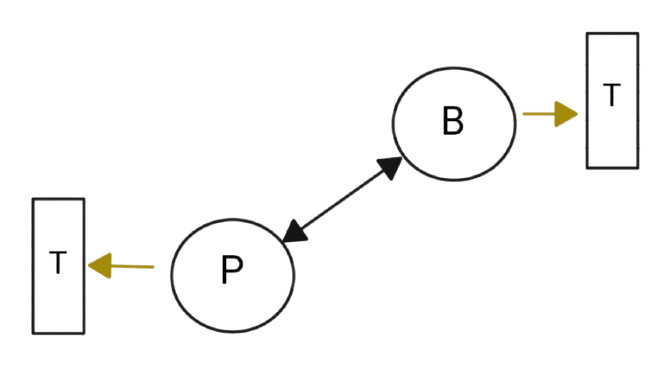
\includegraphics[width=0.50\textwidth]{link.png} % Percorso e dimensioni
    \caption{Astrazione del collegamento tra il bootstrap principale e il backup. La freccia nera rappresenta il collegamento bidirezionale tra i due nodi, utilizzato per monitorarsi a vicenda. Il nodo A rappresenta il Bootstrap principale, mentre il nodo B rappresenta il Backup. Le componenti T rappresentano la tabella distribuita gestita dal Bootstrap.} % Testo sotto l'immagine
    \label{fig:esempio} % Etichetta per riferimenti incrociati
\end{figure}

L'algoritmo utilizza il meccanismo di failover di Erlang, basato su messaggi di \texttt{exit}, per trasferire il controllo al nodo di backup in caso di guasto:
\begin{itemize}
    \item Il nodo principale e il nodo di backup si monitorano a vicenda tramite \textbf{link}. Il nodo di backup viene creato inviando al nodo principale (bootstrap) un messaggio di \textbf{createBackup}, all'interno della funzione che avvia l'intero sistema.
    \item In caso di crash del nodo di bootstrap principale:
    \begin{itemize}
        \item Il nodo di backup assume il ruolo di nodo principale, registrandosi come tale.
        \item Un nuovo nodo di backup viene creato dinamicamente e registrato.
    \end{itemize}
    \item In caso di crash del nodo di backup:
    \begin{itemize}
        \item Il nodo principale ricrea una nuova istanza di backup, registrandola opportunamente.
    \end{itemize}
\end{itemize}

Ovviamente, se un nodo riceve un segnale che l'altro ha effettuato un \texttt{exit}, il nodo in questione gestirà il messaggio senza effettuare anch'esso un \texttt{exit}. Questa scelta è necessaria poiché, essendo il bootstrap un nodo principale, non è possibile lasciare la rete priva di un nodo bootstrap. Segue il codice di implementazione che descrive come il nodo bootstrap gestisce il messaggio di \texttt{exit}.

\textbf{exit}
\begin{lstlisting}
{'EXIT', _, _Reason} ->
    case Role of
        primary ->
            NewBackupPid = spawn_link(node(), fun() ->
                bootstrap_node_loop(rand:uniform(1 bsl 160 - 1), backup)
                    end),
                global:register_name(backup_bootstrap, NewBackupPid),
                bootstrap_node_loop(Id, primary);
        backup ->
            global:unregister_name(backup_bootstrap),
            global:register_name(bootstrap, self()),
            NewBackupPid = spawn_link(node(), fun() ->
                bootstrap_node_loop(rand:uniform(1 bsl 160 - 1), backup)
                end),
            global:register_name(backup_bootstrap, NewBackupPid),
            bootstrap_node_loop(Id, primary)
    end;
\end{lstlisting}

Utilizzando la funzione \textbf{bootstrap:print\_all()}, è possibile visualizzare l'intero contenuto della tabella di Bootstrap. Quest'ultima consente solo operazioni di inserimento; quindi, se un nodo muore, non verrà rimosso dalla tabella. Anche se a un nuovo nodo venisse fornito il PID di uno non più esistente, ciò non causerebbe problemi, poiché il nodo aggiornerà autonomamente la propria \texttt{K\_buckets} con il passare del tempo.

I nodi Bootstrap utilizzano \textbf{Mnesia}, un database distribuito nativo di Erlang, per memorizzare informazioni su tutti i nodi della rete. In particolare:
\begin{itemize}
    \item La tabella \texttt{bootstrap\_table} archivia \texttt{ID} e \texttt{PID}.
    \item Le operazioni su questa tabella sono transazionali, garantendo consistenza anche in presenza di errori.
\end{itemize}
La scelta di utilizzare \texttt{Mnesia} deriva dalla necessità di distribuirne il contenuto tra i vari nodi Bootstrap. Di base, \texttt{Mnesia} garantisce persistenza locale, ma per un corretto funzionamento della rete è necessario eliminare la cartella locale generata da \texttt{Mnesia} per creare nuovamente la rete da zero. In caso contrario, la rete partirebbe considerando nodi creati in precedenza ma non più esistenti, causando conflitti.

Il comportamento generale del Bootstrap è definito dalla funzione \textbf{bootstrap\_node\_loop}, che consente lo scambio dei seguenti messaggi:
\begin{itemize}
    \item \texttt{ping}: stampa a video un messaggio che segnala la ricezione del ping. Il messaggio utilizzato è:\\
    \{ping, From\}.
    \item \texttt{createBackup}: consente la creazione del nodo di backup, ovvero una nuova istanza del nodo principale che ha il compito di monitorarlo. Il messaggio utilizzato è \\
    \{\texttt{createBackup, backupId}\}.
    \item \texttt{enter}: permette a un nuovo nodo, non ancora parte della rete di Kademlia, di effettuare la richiesta di ingresso. Questo passaggio è considerato obbligatorio. Il messaggio utilizzato è \\
    \{\texttt{enter, From}\}.
    \item \texttt{crash}: forza il nodo in questione a effettuare una \texttt{exit}. Il messaggio utilizzato è \\\{\texttt{crash}\}.
    \item \texttt{EXIT}: consente la gestione dell'uscita di un nodo Bootstrap, qualunque sia la causa.
\end{itemize}
\subsubsection{Entrata di un nodo nella rete}
Come affermato precedentemente, qualsiasi nod deve contattare il nodo Bootstrap per fare richiesta di ingresso nella rete Kademlia. Questo viene effettuato inviando il seguente messaggio:
\begin{lstlisting}
global:whereis_name(bootstrap) ! {enter, Nodo}.
\end{lstlisting}
Dove, \texttt{Nodo} non è altro che il nodo creato in precedenza. Una volta ricevuto il messaggio, il bootstrap inserirà il nodo nella sua bootstrap\_table e fornirà al nodo appena entrato la lista di k\_buckets. La funzione che si occupa della creazione della k\_buckets è chiamata \textbf{get\_4\_buckets/1}:

\begin{lstlisting}
get_4_buckets(NodeId) ->
    Tran = fun() ->
        mnesia:foldr(
            fun(#bootstrap_table{id = Id, pid = Pid}, Acc) -> 
            case Id == NodeId of
                true ->
                    Acc;
                false ->
                  Distance=binary_xor(NodeId, Id),
                  Acc ++ [{Distance, Id, Pid}]
            end
        end,
        [],
        bootstrap_table
    )
    end,
    {atomic, AllRecords} = mnesia:transaction(Tran),
    SortedRecords = lists:sort(fun({D1,_,_},{D2,_,_})->D1<D2 end, AllRecords),
    case SortedRecords of
        [] ->
            [];
        [_] ->
            SortedRecords;
        _ ->
            ClosestTwo = lists:sublist(SortedRecords, 2),
            TotalNodes = length(SortedRecords),
            MiddleNodeIndex =
                case TotalNodes > 2 of
                    true -> round(TotalNodes / 2);
                    false -> 1
                end,
            MiddleNode = lists:nth(MiddleNodeIndex, SortedRecords),
            FarthestNode = lists:last(SortedRecords),
            UniqueNodes = lists:usort(ClosestTwo ++ [MiddleNode, FarthestNode]),
            lists:sublist(UniqueNodes, 4)
    end.
\end{lstlisting}

\subsection{Considerazioni}
L'implementazione così descritta, riesce a presentare queste proprietà:
\begin{itemize}
    \item \textbf{Concorrenza e scalabililità}:
    \begin{itemize}
        \item Ogni nodo è un processo indipendente, sfruttando il modello ad attori per una gestione efficiente della concorrenza.
        \item L'approccio a bucket consente la scalabilità per reti di grandi dimensioni.
    \end{itemize}
    \item \textbf{Robustezza}:
    \begin{itemize}
        \item Il sistema tollera il fallimento dei nodi, garantendo che la rete rimanga operativa anche in condizioni avverse.
    \end{itemize}
    \item \textbf{Estensibilità}:
    \begin{itemize}
        \item La modularità del codice consente di aggiungere nuove funzionalità senza interrompere il comportamento esistente.
    \end{itemize}
\end{itemize}

\section{Creazione e avvio della rete}
Per creare da zero e avviare la rete Kademlia descritta, vanno seguiti i seguenti passi:
\begin{enumerate}
    \item Controllare che non sia presente la cartella riferita ad Mnesia;
    \item Avviare Erlang su due terminali distinti. Ciascuna istanza di Elang deve avere il parametro \texttt{sname} diverso;
    \item Effettuare dal nodo 1 una \texttt{spawn('nodo2@...', fun() -> ok end.)} per far communicare le due istanze;
    \item \texttt{bootstrap:start\_system(self())}.
    \item Creiamo un nuovo nodo che però ancora non farà parte della rete di Kademlia:\\ \texttt{\{\_, Nodo1\} =\\nodo:new\_kademlia\_node(self())}.
    \item \texttt{global:whereis\_name(boostrapt) ! \\ \{enter, Nodo1\}}.
\end{enumerate}
\section{Esperimenti e Risultati}
In questa sezione vengono descritti gli esperimenti svolti e i relativi risultati. Le simulazioni sono state effettuate con una rete inizializzata a 0 nodi, 100 nodi e 500 nodi. Le operazioni princi-pali testate includono l'inserimento di nodi, la ricerca (\texttt{find\_node} e \texttt{find\_value}), e il ping. I risultati, espressi in microsecondi, sono riassunti nelle tabelle seguenti.
\subsection{Metriche di inserimento e ricerca}
La Tabella 1 riporta i tempi medi di esecuzione per l'inserimento di nodi e le operazioni di ricerca \\(\texttt{find\_node} e \texttt{ping}) nelle diverse configurazioni della rete.
\begin{table}[htbp] 
    \centering 
    \begin{tabular}{|c|c|c|c|} 
    \hline
        & \multicolumn{3}{|c|}{Numero di nodi} \\
        \hline
        Operazione & 0  & 100  & 500  \\
        \hline
        Inserimento & 2560 & 119,808 & 3,302,607 \\ 
        \hline
        \texttt{find\_node} & - & 10,957 & 5734 \\ 
        \hline
        \texttt{ping} & - & 8500 & 7373 \\
        \hline 
    \end{tabular} 
    \caption{Tempi medi per inserimento e ricerca (\texttt{find\_node}, \texttt{ping}), in microsecondi.} 
    \label{tab:tempi medi} 
\end{table}
Per quanto riguarda il tempo dello \textbf{store} (inserimento di un valore all'interno di un nodo), il processo risulta molto rapido, con una media di 3175 microsecondi. Questo tempo non dipende dal numero di nodi presenti nella rete, grazie all'implementazione ottimizzata del sistema.
\subsection{Efficienza di \texttt{find\_value}}
La nostra implementazione di Kademlia dimostra un'elevata efficienza nell'operazione \texttt{find\_value}. I nodi inviano periodicamente (ogni 30 secondi) il loro contenuto (chiavi e valori) ai nodi raggiungibili. Questo meccanismo consente di mantenere un tempo di ricerca costante, indipendentemente dal numero di nodi nella rete.
\begin{table}[htbp] 
    \centering 
    \begin{tabular}{|c|c|c|c|} 
        \hline
        & \multicolumn{3}{|c|}{Numero di nodi} \\
        \hline 
        Operazione & 0 & 100 & 500 \\ 
        \hline 
        \texttt{find\_value} & - & 102 & 102 \\ 
        \hline 
    \end{tabular} 
    \caption{Tempo medio di esecuzione di \texttt{find\_value}, in microsecondi.} \label{tab:find_value} 
\end{table}
\subsection{Tempi di Ripristino del Bootstrap}
In caso di fallimento di un nodo \textbf{Bootstrap}, il sistema è progettato per garantire un ripristino rapido ed efficiente come riportato nella Tabella 3.
\begin{table}[!htbp] 
    \centering 
    \begin{tabular}{|c|c|} 
        \hline 
        Nodo Bootstrap & Tempo Medio [$\mu$s] \\ 
        \hline 
        Principale & 1228 \\ 
        \hline 
        Backup & 1024 \\ 
        \hline 
    \end{tabular} 
    \caption{Tempi medi di ripristino in caso di fallimento del Bootstrap.} \label{tab:Bootstrap} 
\end{table} 
Questi valori sono stati ottenuti simulando volutamente un fallimento del nodo di Bootstrap mediante il comando \texttt{crash}. Quest'ultimo genera un messaggio di \texttt{exit}, attivando il meccanismo di ripristino implementato nella logica del sistema.
\printbibliography
\end{document}
